We observed in the previous section that the number of staffs and meeting rooms varies from building to building. This presents an opportunity for us to consider if the current allocation for meeting rooms can offer flexibility for staffs (i.e. if meeting rooms for that building are fully booked, can the staff find another meeting room nearby?). In this section, we map the staffs and meeting rooms data with building outlines and building GPS using QGIS. 

QGIS provides visualisation of the “heat-map” of the average meeting room capacity per staff, which is calculated using the total capacity of meeting rooms divided by the amount of staff as shown in Figure 10. The dark (blue) cell represents high availability and the green colour indicates that either the meeting room or staff number is zero. Using this analysis, we can deduce following results:

\begin{itemize}
    \item \texttt{Doug McDonell building(168)}, \texttt{11 Barry Street(266)} and \texttt{Law building(106)} have a significant number of staffs and therefore stronger demand for meeting rooms. The following analysis assumes that 3-minute walk is the distance people are willing to walk. And based on the average walking speed of an adult, a three-minute walk is about 240 meters.
    
    \item For staffs in \texttt{Doug McDonell(168)}, \texttt{Old Engineering School(173)}and \texttt{Walter Boas(163)} are merely 150 meters away and both buildings have a comparatively small number of staffs and high meeting room capacities.
    
    \item \texttt{11 Barry Street(266)} is near \texttt{Law building(106)}, and other surrounding buildings such as \texttt{Kwong Lee Dow building(263)}, \texttt{The Spot(110)} and \texttt{FBE building(105)} also have lots of staffs.
    
    \item Also, all of these buildings have low ratios, indicating that those staffs may need to use meeting rooms in other buildings as well.  Choices are including \texttt{MDHS(207)}, \texttt{Statistical Consulting Center(394)} and \texttt{University Business Service building(384)}, however, their meeting rooms capacity is around 20, and it might be difficult for them to support those high-demand buildings nearby.
\end{itemize}
   
   
\begin{figure}[H]
    \centering
    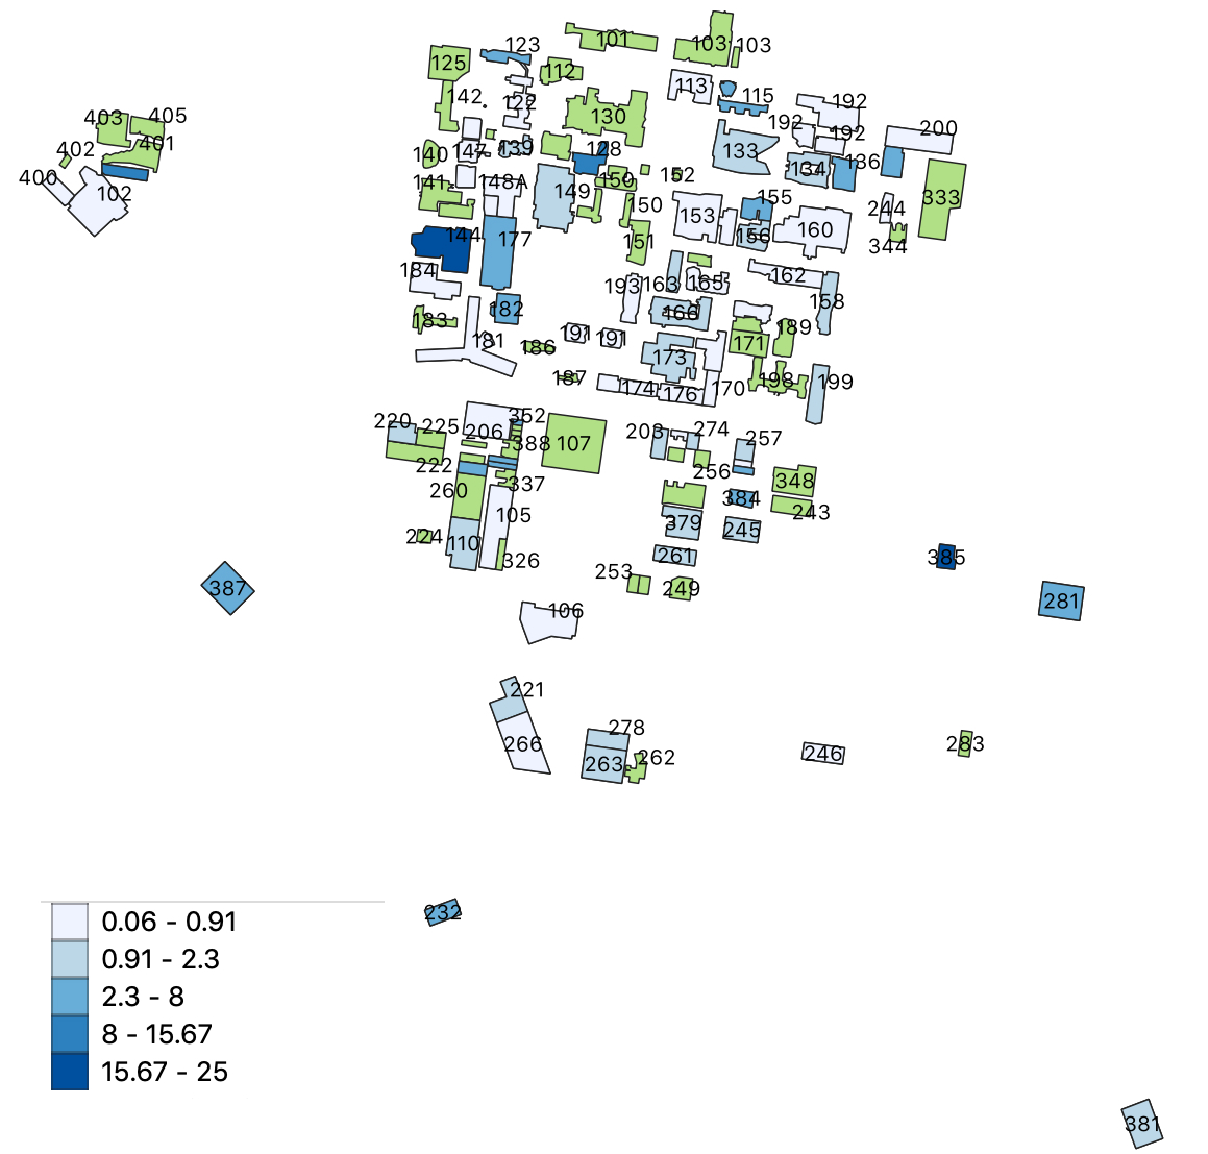
\includegraphics[width=15cm]{resources/images/capacity_meetingroom.pdf}
    \caption{Spatial Analysis: Capacity of meeting rooms with respect to Staff}
    \label{mr_staff}
\end{figure}
